
\section{Heat, Temperature, and Internal Energy}

Name \rule{2.0in}{0.1pt}\hfill{}Section \rule{1.0in}{0.1pt}\hfill{}Date
\rule{1.0in}{0.1pt}

\textbf{Objective}

To investigate the relationship between heat and temperature.

\textbf{Apparatus}

\begin{itemize}
\item Glass beaker 
\item Glass stirring rod
\item Hot plate
\item Ice
\item Data Studio software and temperature probe
\item Clamp and stand
\end{itemize}
\textbf{Temperature of a Substance as a Function of Heat Transfer}

As part of our quest to understand heat energy transfer, temperature,
and internal energy of a substance, let's consider the temperature
change as ice is changed to water and then to steam.

\textbf{Activity 1: Predicting T vs. t for Water} 

Suppose you were to add heat at a constant rate to a container of
ice water at 0\( ^{\circ } \)C until the water begins to boil. Sketch
the predicted shape of the heating curve on the graph below using
a dashed line. Mark the points at which the ice has melted and the
water begins to boil.

\vspace{0.3cm}
{\centering 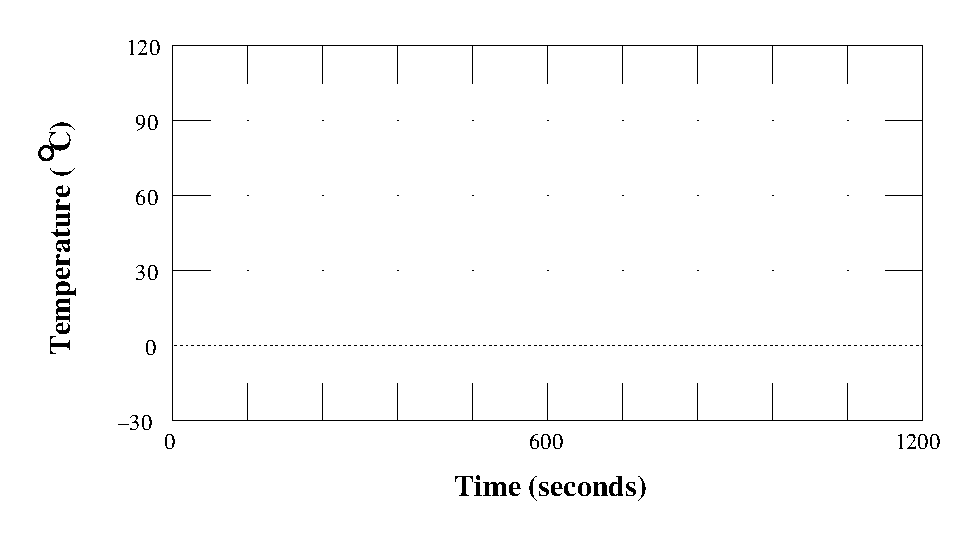
\includegraphics{heat_temp_int_energy_fig_1.eps} \par}
\vspace{0.3cm}

\newpage

\textbf{Activity 2: Measuring T vs. t for Water} 

(a) To test your prediction: 

\begin{enumerate}
\item Fill the glass beaker one third full of ice and set it on top of the hot plate.
\item Suspend the temperature probe so that the end is submerged in the ice but not touching the side or bottom of the beaker. You will need to use the clamp and stand to do this. BE SURE THE WIRE FROM THE TEMPERATURE PROBE IS NOT TOUCHING THE HOT PLATE OR GLASS BEAKER. Also, be sure the temperature probe is attached to port ``A'' of the Pasco interface. Let set for 60 seconds so temperature probe can come to equilibrium with the ice.
\item Open the \textit{Heat, Temp, \& Internal Energy} application in the
132 Workshop folder under \textit{Physics Applications}.
\item Turn on the hot plate to about 6 and click the
\textbf{Start} button on the monitor to begin recording data. The temperature of the water will be recorded on the graph shown on the monitor. Stir often to keep ice against the temperature probe.
\item When ice begins to turn to water, stir at about 1 minute intervals. When all ice is melted, there is no need to stir any further.
\item After the water begins to boil, keep hot plate on for a ninute or two as temperature flattens at 100 degrees.
\item Stop data collection using the \textbf{Stop} button and turn off hot plate.
\item Sketch the shape of the measured heating curve on the above graph
using a solid line. Ignore small variations due to noise and uneven
heating. Mark the points at which the ice has melted and the water
begins to boil.
\end{enumerate}
(b) Does your prediction agree with the measured heating curve? If
not, what are the differences?
\vspace{15mm}

(c) What is the relationship between the temperature and the added
heat while the ice is melting?
\vspace{15mm}

(d) What is the relationship between the temperature and the added
heat after the ice has melted, but before the water begins to boil?
\vspace{15mm}

(e) What is the relationship between the temperature and the added
heat while the water is boiling?
\vspace{15mm}

(f) If there are regions of the heating curve in which the temperature
is not changing, what do you think is happening to the added heat
in these regions?\vspace{15mm}

